\hypertarget{project-popularity}{%
\subsubsection{Project Popularity}\label{project-popularity}}

Question: How popular is an open source project?

\hypertarget{description}{%
\paragraph{Description}\label{description}}

Project popularity can be measured by how much activity is visible
around a project. Popularity has a positive feedback loop in which more
popular projects get more attention, attract more users or developers,
and see increases in popularity, spinning the popularity wheel.

Project popularity may be used as a proxy for understanding project
value because open source project economic value is hard to measure, due
to a lack of available usage or sales information for open source
projects.

\hypertarget{objectives}{%
\paragraph{Objectives}\label{objectives}}

In a quest to earn a living wage, and to maximize future employment
opportunities, workers may be interested in knowing which projects are
growing and are underserved. Similarly, from an organizational
perspective, knowing which projects are highly used can be helpful in
knowing which projects might be worth investing in. The Project
Popularity metric can be used to identify the trajectory of a project's
development.

\hypertarget{implementation}{%
\paragraph{Implementation}\label{implementation}}

The project popularity metric is often considered with changes over
time. There are numerous example vectors to consider when measuring
project popularity based on the number of:

\begin{enumerate}
\def\labelenumi{\arabic{enumi}.}
\tightlist
\item
  Social media mentions
\item
  Forks
\item
  \href{https://chaoss.community/metric-change-requests/}{Change
  requests}
\item
  \href{https://chaoss.community/metric-issues-new/}{New Issues}
\item
  Stars, badges, likes
\item
  \href{https://chaoss.community/metric-new-contributors/}{New
  contributors}
\item
  \href{https://chaoss.community/metric-organizational-diversity/}{Organizational
  Diversity}
\item
  Job postings requesting skills in project
\item
  Conversations within and outside of project
\item
  Clones
\item
  Followers
\item
  Downstream dependencies
\item
  People attending events that focus on a project
\end{enumerate}

\hypertarget{visualizations}{%
\subparagraph{Visualizations}\label{visualizations}}

Issues and reviews (change requests) visualization from Cauldron
(GrimoireLab):

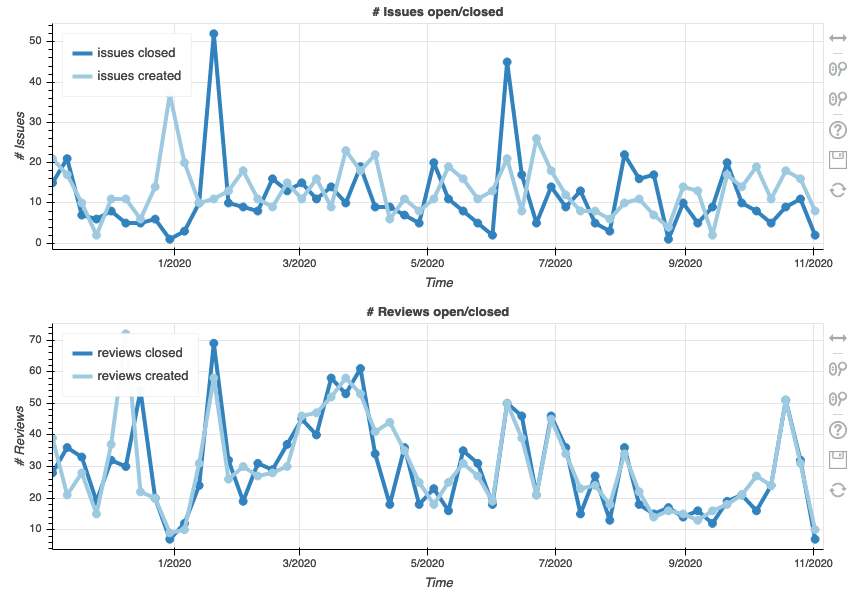
\includegraphics{images/project-popularity_issues-and-reviews.png}

Kubernetes project popularity statistics from DevStats:

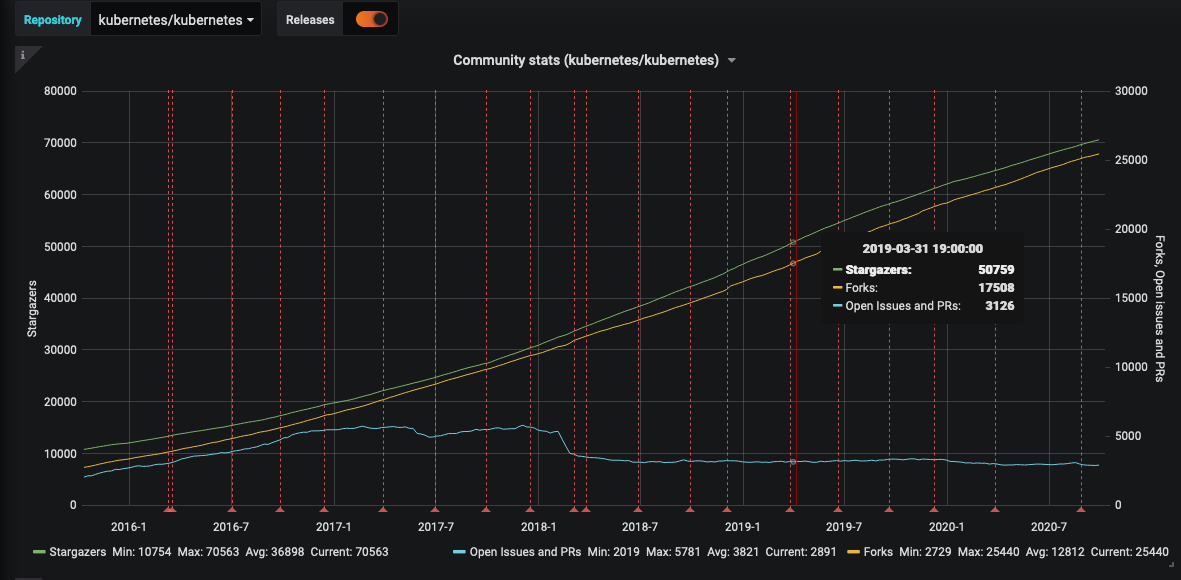
\includegraphics{images/project-popularity_kubernetes.png}

\hypertarget{tools-providing-the-metric}{%
\subparagraph{Tools Providing the
Metric}\label{tools-providing-the-metric}}

\begin{itemize}
\tightlist
\item
  \href{https://github.com/chaoss/augur}{Augur}
\item
  \href{https://chaoss.github.io/grimoirelab/}{GrimoireLab}
\item
  \href{https://cauldron.io/}{Cauldron}
\end{itemize}

\hypertarget{references}{%
\paragraph{References}\label{references}}

\begin{itemize}
\tightlist
\item
  \href{http://blog.honeypot.io/most-exciting-open-source-projects-2018/}{Popular
  OpenSource Projects}
\item
  \href{https://isitmaintained.com/}{Is It Maintained?}
\item
  \href{https://github.blog/2018-02-08-open-source-project-trends-for-2018/}{Open
  Source Project Trends}
\item
  \href{https://www.payscale.com/research/US/Skill=Kubernetes/Salary}{Kubernetes
  Salary}
\end{itemize}
